\documentclass[12pt]{scrartcl}
\usepackage{geometry}
\usepackage{amsmath}
\usepackage[english]{babel}
\usepackage{fontspec}
\usepackage{svg}
\usepackage{hyperref}
\setmainfont{Liberation Serif}
\geometry{a4paper,left=30mm,right=30mm, top=2cm, bottom=2cm}

\begin{document}
  \title{Project Work at MPIK}
  \subtitle{Temperature control system}
  \date{}
  \author{Stefan Dickopf}
  \maketitle

  \section{Experimental setup}
    A temperature sensor, a heater and a cooler are to be connected to a Arduino
    board. In order for it to work we need to have shifters for the voltage
    range to fit the inputs/outputs on the Arduino. This was first done by
    Vanessa Scheller using cables and a breadboard, I took her design and
    reworked it to be used on a milled circuit board and SMD parts.

    \subsection{Temperature sensor circuit}
      The circuit for the temperature sensor looks as follows:
      \begin{figure}[h]
        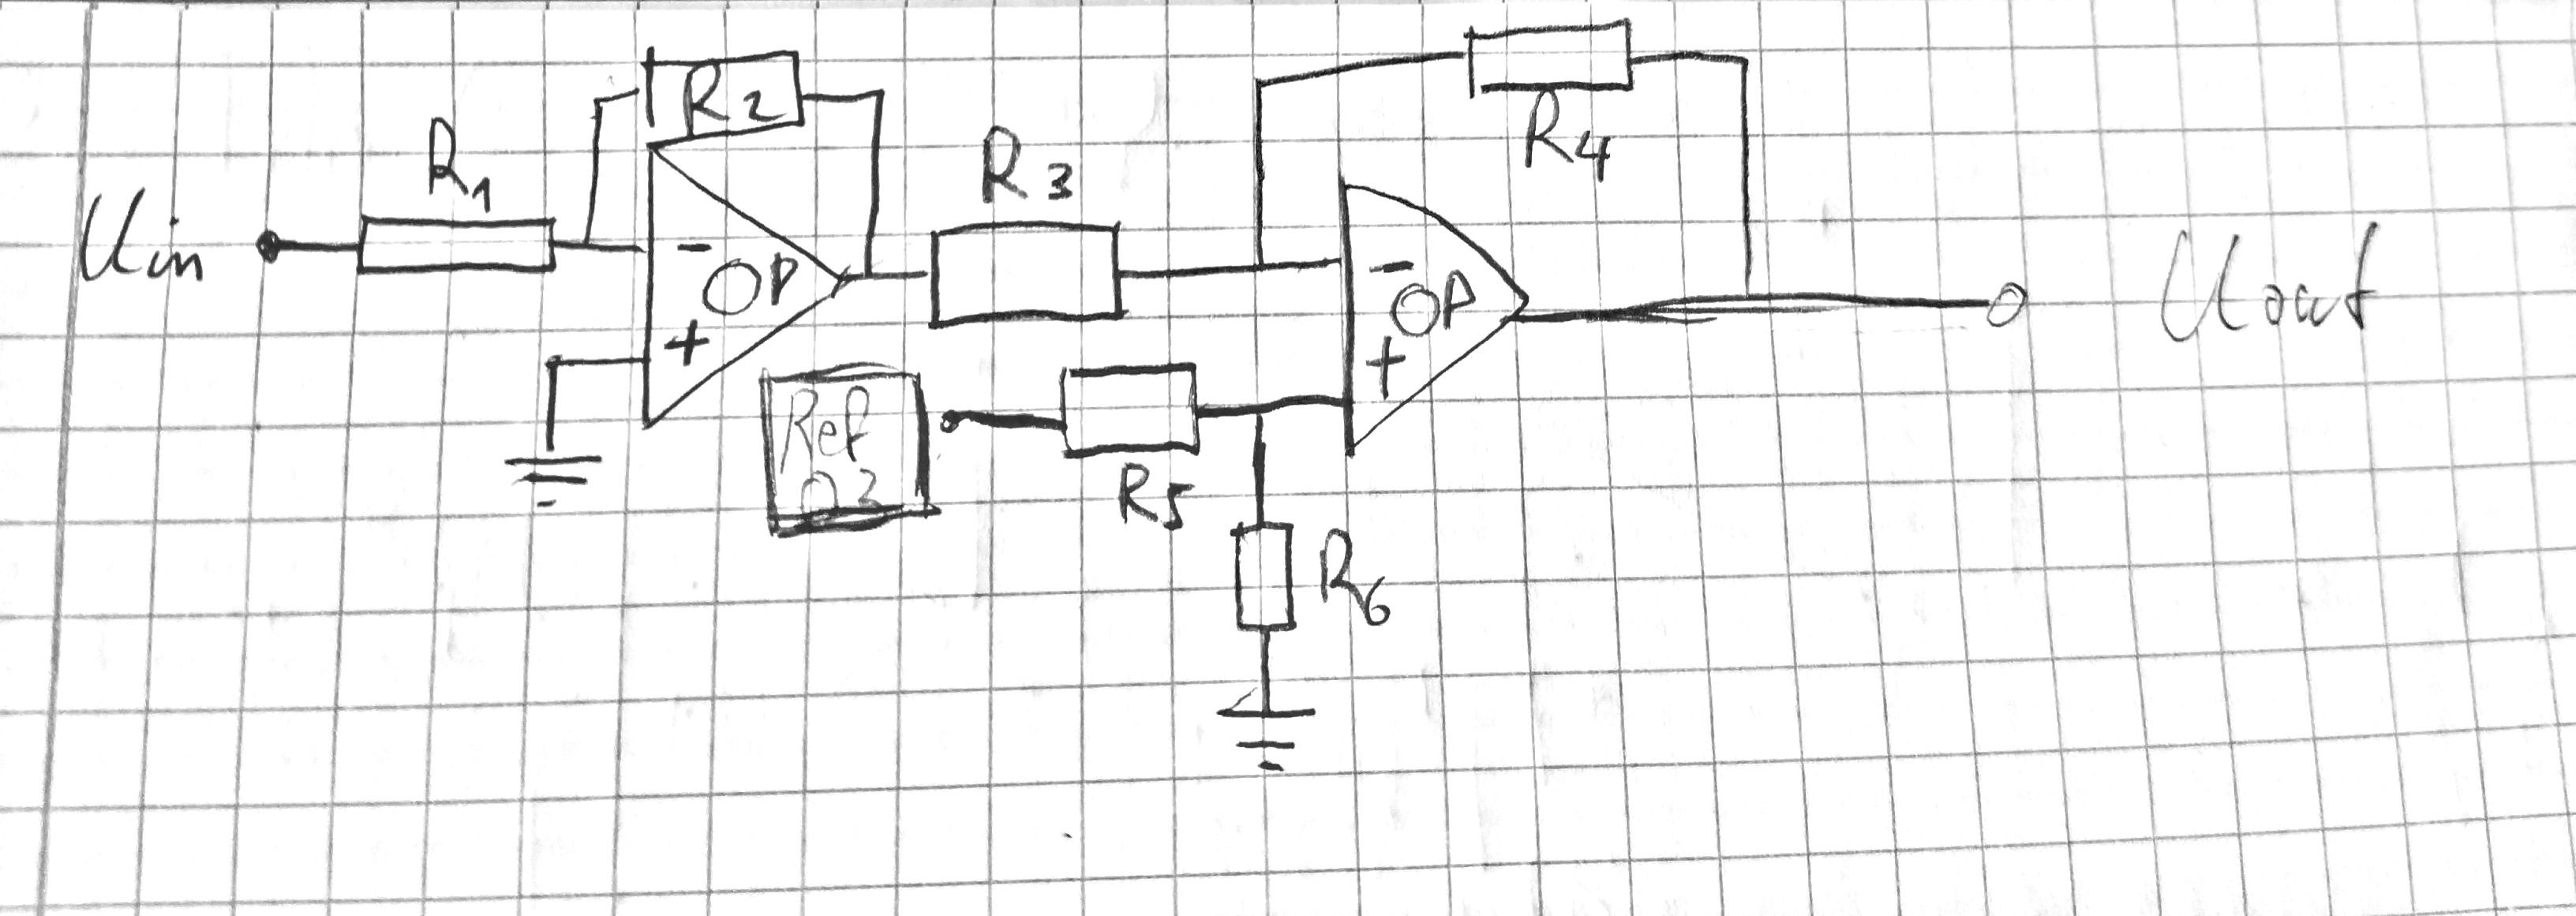
\includegraphics[width = \textwidth]{circ.png}
        \caption{temp. sensor shifter circuit}
        \label{fig1}
      \end{figure}
      \\The input range from the temperature sensor we are interested in is
      $$-1.6V < U_{in} < 1.6V$$
      The supply voltage of the op-amps is 15V. We want to have a cutoff after
      the first op-amp at the input range boundaries. This can be achieved with
      setting the amplification factor with $R_1$ and $R_2$. The output range
      should equal the input range of the Arduino analogue input which goes form
      0-3.3V. The values found for the resistances are as follows (in $k\Omega$):
      \\\\
      $R_1 = 15k\Omega$ \\ $R_2 = 133k\Omega$ \\ $R_3 = 133k\Omega$ \\
      $R_4 = 12k\Omega + 10k\Omega$(potentiometer) \\ $R_5 = 10k\Omega$ \\
      $R_6 = 15k\Omega + 5k\Omega$(potentiometer) \\
      This gives to following response to the input Voltage $U_{in}$
      \begin{figure}[h]
        \includesvg[,width = \textwidth,svgpath=./plots/]{plotimage}
        \caption{temp. sensor shifter circuit}
        \label{fig2}
      \end{figure}

\end{document}
